\documentclass{article}
\usepackage[utf8]{inputenc}
%\usepackage{preamble}
\usepackage{graphicx}
\usepackage{float}
\usepackage{geometry}
\geometry{
    %paperwidth=6.0in,
    %paperheight=9.0in,
    width=5.5in,
    height=8.5in,
    hmarginratio=1:1,  % 3:2 for binding offset
    vmarginratio=1:1,
    includehead=true,
    headheight=15pt
}

% index with headings
\usepackage{imakeidx}
\makeindex[options= -s headings.ist]

% paragraph spacing
\setlength{\parindent}{0pt}                      % 17.62482pt
\setlength{\parskip}{12pt plus 4pt minus 4pt}    % 0.0pt plus 1.0pt
\linespread{1.05}
\def\arraystretch{1.5}

% list spacing
\setlength{\topsep}{5pt plus 2pt minus 3pt}      % 10.0pt plus 4.0pt minus 6.0pt
\setlength{\partopsep}{-6pt plus 2pt minus 2pt}  %  3.0pt plus 2.0pt minus 2.0pt
\setlength{\itemsep}{0pt}                        %  5.0pt plus 2.5pt minus 1.0pt

% these are copied from tex/latex/base/book.cls
% all I changed is afterskip
\makeatletter
\renewcommand{\section}{\@startsection{section}{1}{\z@}%
    {-3.5ex \@plus -1ex \@minus -.2ex}%
    {0.7ex \@plus.2ex}%
    {\normalfont\Large\bfseries}}
\renewcommand\subsection{\@startsection{subsection}{2}{\z@}%
    {-3.25ex\@plus -1ex \@minus -.2ex}%
    {0.3ex \@plus .2ex}%
    {\normalfont\large\bfseries}}
\renewcommand\subsubsection{\@startsection{subsubsection}{3}{\z@}%
    {-3.25ex\@plus -1ex \@minus -.2ex}%
    {0.3ex \@plus .2ex}%
    {\normalfont\normalsize\bfseries}}
\makeatother

% table of contents vertical spacing
\usepackage{tocloft}
\setlength\cftparskip{8pt plus 4pt minus 4pt}

% balanced index with TOC entry
\usepackage[totoc]{idxlayout}

% The following line adds a little extra space to the column
% in which the Section numbers appear in the table of contents
\makeatletter
\renewcommand{\l@section}{\@dottedtocline{1}{1.5em}{3.0em}}
\makeatother

% customize page headers
\usepackage{fancyhdr}
\pagestyle{fancyplain}
\renewcommand{\chaptermark}[1]{\markboth{Chapter \thechapter ~~ #1}{}}
\renewcommand{\sectionmark}[1]{\markright{\thesection ~~ #1}}
\lhead[\fancyplain{}{\bfseries\thepage}]%
      {\fancyplain{}{\bfseries\rightmark}}
\rhead[\fancyplain{}{\bfseries\leftmark}]%
      {\fancyplain{}{\bfseries\thepage}}
\cfoot{}
%\usepackage[mmddyyyy]{datetime}
%\rfoot{\textcolor{gray}{\tiny \thetitle, \theversion, \today}}

%% tweak spacing of figures and captions
%\usepackage{floatrow}
%\usepackage{caption}
%\captionsetup{
%    font=small,
%    labelformat=empty,
%    justification=centering,
%    skip=4pt
%}

% colors for code listings and output
\usepackage{xcolor}
\definecolor{bgcolor}{HTML}{FAFAFA}
\definecolor{comment}{HTML}{007C00}
\definecolor{keyword}{HTML}{0000FF}
\definecolor{strings}{HTML}{B20000}

% syntax highlighting in code listings
\usepackage{textcomp}
\usepackage{listings}
\lstset{
    language=java,
    basicstyle=\ttfamily,
    backgroundcolor=\color{bgcolor},
    commentstyle=\color{comment},
    keywordstyle=\color{keyword},
    stringstyle=\color{strings},
    columns=fullflexible,
    emph={label},  % keyword?
    keepspaces=true,
    showstringspaces=false,
    upquote=true,
    xleftmargin=15pt,  % \parindent
    framexleftmargin=3pt,
    aboveskip=\parskip,
    belowskip=\parskip
}

% code listing environments
\lstnewenvironment{code}
{\minipage{\linewidth}}
{\endminipage}
\lstnewenvironment{stdout}
{\lstset{commentstyle=,keywordstyle=,stringstyle=}\minipage{\linewidth}}
{\endminipage}

% interactive code listing
\lstnewenvironment{trinket}[2][400]
{\minipage{\linewidth}}
{\endminipage}

% inline syntax formatting
\newcommand{\java}[1]{\lstinline{#1}}%{

% prevent hyphens in names
\hyphenation{DrJava}
\hyphenation{GitHub}
\hyphenation{Javadoc}

% pdf hyperlinks, table of contents, and document properties
\usepackage{hyperref}

% add dot after numbers in pdf bookmarks
\makeatletter
\renewcommand{\Hy@numberline}[1]{#1. }
\makeatother

\makeatletter
%\renewcommand{\@seccntformat}[1]{}
% \newcommand{\java}[1]{{\texttt #1}}%{

% \lstset{language = Java, numbers = none, basicstyle=\scriptsize\ttfamily, frame=lines, numberstyle=\tiny, breaklines=true, tabsize = 4, backgroundcolor=\color{white}, captionpos=b}

%frame=lines
\makeatother

\title{Simplified Predictive Modeling In Java \vspace{-8mm}}
\author{}
\date{}

\begin{document}

\maketitle

\section{Introduction}
The goal of this tutorial is to provide example code for predictive modeling in Java, using three custom-built classes: \verb|Data|, \verb|Plot|, and \verb|LearningMachine|. These classes are designed so that the user does not have to worry about the details of the code, but instead can focus on learning the basics of predictive modeling. 

\section{The Data Class}
In this example, we will be using the \verb|ICU_data.csv| dataset. Each row of the CSV contains data on a single patient. First, we read the data into the \verb|Data| class:

\begin{lstlisting}
String file = "ICU_Data.csv";
Data d = new Data(file);
\end{lstlisting}

The \verb|Data| constructor reads in a file location or a URL and stores the data in a \verb|String[][]| object. After storing the first row of the CSV as the instance variable \verb|String[][] headers|, it then randomly splits the data into training/testing/validation sets and stores them as the instance variables \verb|String[][] train|, \verb|String[][] test|, and \verb|String[][] valid|. 

Let's take a look at the first few headers for our dataset.
\begin{lstlisting}
for (int i = 1; i < 6; i++) {
    System.out.print(d.headers[i] + " ");
}
\end{lstlisting}

This gives us an output of: 
\begin{lstlisting}
Age DiasABP FiO2 GCS Gender 
\end{lstlisting}

The last column of our dataset is the binary classification variable we want to predict - whether or not the patient died in the ICU.

\begin{lstlisting}
System.out.println(d.headers[d.headers.length - 1]);
\end{lstlisting}

This gives us an output of: 
\begin{lstlisting}
In-hospital_death
\end{lstlisting}

The \verb|Data| class also has three methods for obtaining a subset of the data according to a specific filter: \verb|getRows|, \verb|getCols|, and \verb|convertToDouble|. For example, suppose we want to only look at the patients in the training data who are male. We can use the \verb|getRows| method: 

\begin{lstlisting}
int genderIndex = Arrays.asList(d.headers).indexOf("Gender");
String[][] male = d.getRows(d.train, genderIndex, "M");
String[][] female = d.getRows(d.train, genderIndex, "F");
\end{lstlisting}

If we wanted the GCS (Glasgow Coma Scale) score as well as the age of all the patients in the training data, we can use the \verb|getCols| method:

\begin{lstlisting}
int ageIndex = Arrays.asList(d.headers).indexOf("Age");
int GCSIndex = Arrays.asList(d.headers).indexOf("GCS");
String[][] twoCols = d.getCols(d.train, new int[] {ageIndex, GCSIndex});
\end{lstlisting}

Finally, suppose we just wanted the age of the all the training data patients, as well as separate age data for each gender. Since we know \verb|age| is a numerical variable, we can use the \verb|convertToDouble| method, which gives us a \verb|double[]| rather than a \verb|String[]|.

\begin{lstlisting}
double[] ages = d.convertToDouble(d.train, ageIndex);
double[] agesM = d.convertToDouble(male, ageIndex);
double[] agesF = d.convertToDouble(female, ageIndex);
\end{lstlisting}

\section{The Plot Class}
The \verb|Plot| class contains two methods: \verb|plotHistogram| and \verb|plotRates|. The class uses the \verb|JFreeChart| Java library to generate graphs of our data. For example, suppose we want to visualize the \verb|agesM| and \verb|agesF| arrays in two histgrams:

\begin{lstlisting}
double[][] allAges = {agesM, agesF};
String[] legend = {"Male", "Female"};
Plot.plotHistogram(allAges, legend, "ICU_agesG.png", 
	"Age Distribution of Patients by Gender", "Age", "Frequency");
\end{lstlisting}

This will produce the following output:
\begin{figure}[H]
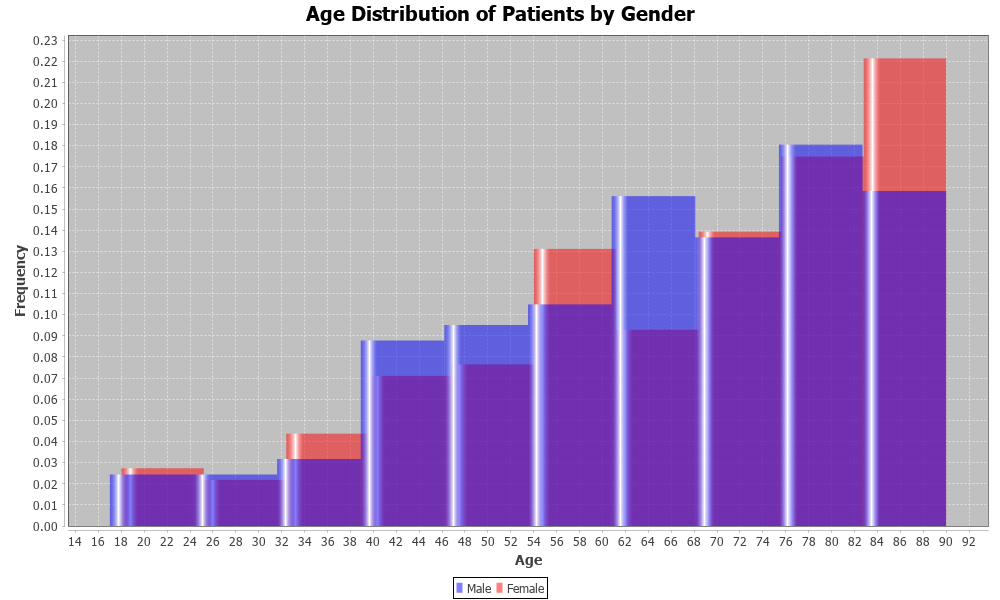
\includegraphics[scale=0.3]{ICU_agesG.png}
\centering
\end{figure}

The \verb|plotRates| method also can plot multiple line charts on the same graph. Below is a simple example on how to call the \verb|plotRates| method:

\begin{lstlisting}
double[] sampleX = {1, 5};
double[] sampleY1 = {2, 2};
double[] sampleY2 = {3, 7};
double[][] allY = {sampleY1, sampleY2};
String[] seriesNames = {"Series 1", "Series 2"};
Plot.plotRates(sampleX, allY, seriesNames, "sample_line_graph.png", 
		"Sample Line Graph", "x", "y");
\end{lstlisting}

\begin{figure}[H]
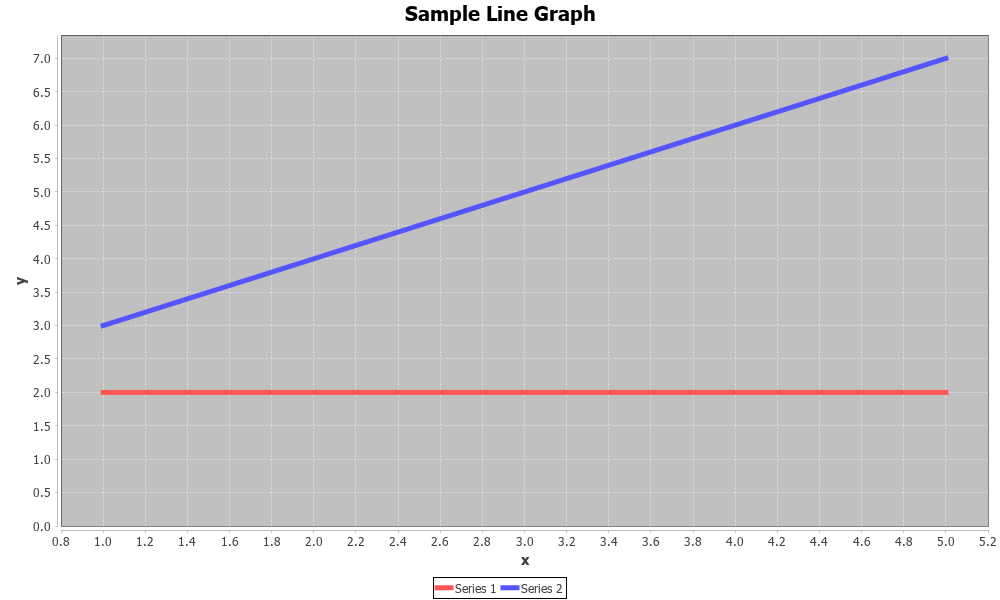
\includegraphics[scale=0.3]{sample_line_graph.png}
\centering
\end{figure}


\section{The LearningMachine Class}
The \verb|LearningMachine| class uses the \verb|Weka| library, which contains tools for data mining and machine learning algorithms. \verb|LearningMachine| has the instance variable \verb|fit|, which is the \verb|Weka| classifier for the model. The \verb|LearningMachine| constructor has the following parameters:

\begin{itemize}
    \item \verb|String[] preds|: the names of the variables the model should use
    \item \verb|Data d|: the \verb|Data| object that \verb|trainData| comes from
    \item \verb|String[][] trainData|: the data used to build the model
\end{itemize}  

For example, if we want to build a classifier using \verb|Age| and \verb|GCS| as predictor variables, with the goal to predict \verb|In-hospital_death|:

\begin{lstlisting}
String[] preds = {"Age", "GCS", "In-hospital_death"};
LearningMachine model = new LearningMachine(preds, d, d.train);
System.out.println(model.fit);
\end{lstlisting}

This outputs the coefficients of our model, as well as the odds ratio:
\begin{lstlisting}
Logistic Regression with ridge parameter of 1.0E-8
Coefficients...
               Class
Variable           0
====================
Age          -0.0359
GCS           0.2404
Intercept    -0.1952


Odds Ratios...
               Class
Variable           0
====================
Age           0.9647
GCS           1.2717
\end{lstlisting}

\verb|LearningMachine| has two \verb|predict| methods, both with essentially the same function. One returns the model's predicted probability of death for a sample patient, while the other does this for multiple patients.

Suppose we have a 45-year-old patient with a GCS score of 7. To see what the model predicts the probability of this patient dying in the ICU, we have:

\begin{lstlisting}
double prob = model.predict(new String[] {"45", "7"}, preds);
System.out.println(prob);
\end{lstlisting}

This gives us an output of:
\begin{lstlisting}
0.46771888210572526
\end{lstlisting}

Note that the first parameter in \verb|predict| is a \verb|String[]| object, even though both of our predictor variables are of type \verb|double|. This is to allow categorical variables to be used in other potential models. 

Now, suppose we want to see what the model predicts on our entire validation set. We can use the other \verb|predict| method as follows:

\begin{lstlisting}
double probs[] = model.predict(d.valid, preds);
System.out.println("Validation set size: " + d.valid.length);
System.out.println("probs[] array length: " + probs.length);
\end{lstlisting}

Our output is:
\begin{lstlisting}
Validation set size: 166
probs[] array length: 166
\end{lstlisting}

We see that both arrays are the same length - for the patient in row \verb|i| of the validation set, our model's predicted probability for their death in the ICU is \verb|probs[i]|. 
\end{document}